%%%%%%%%%%%%%%%%%%%%%%%%%%%%%%%%%%%%%%%%%%%%%%%%%%%%%%%%%%%%%%%%%%%%%%%%%%%% 
% AGUJournalTemplate.tex: this template file is for articles formatted with LaTeX
%
% This file includes commands and instructions
% given in the order necessary to produce a final output that will
% satisfy AGU requirements, including customized APA reference formatting.
%
% You may copy this file and give it your
% article name, and enter your text.
%
% guidelines and troubleshooting are here:

%% To submit your paper:
\documentclass[draft]{agujournal2019}
\usepackage{url} %this package should fix any errors with URLs in refs.
\usepackage{lineno}
\usepackage{placeins}
\usepackage{amsmath}
\usepackage{makecell}

\usepackage[inline]{trackchanges} %for better track changes. finalnew option will compile document with changes incorporated.
\usepackage{soul}
\linenumbers
%% make line numbers work with amsmath
% https://tex.stackexchange.com/questions/461186/how-to-use-lineno-with-amsmath-align
\usepackage{lineno}   %% <- no mathlines option
\usepackage{amsmath}  %% <- after lineno
\usepackage{etoolbox} %% <- for \cspreto, \csappto

%% Patch 'normal' math environments:
\newcommand*\linenomathpatch[1]{%
  \cspreto{#1}{\linenomath}%
  \cspreto{#1*}{\linenomath}%
  \csappto{end#1}{\endlinenomath}%
  \csappto{end#1*}{\endlinenomath}%
}

\linenomathpatch{equation}
\linenomathpatch{gather}
\linenomathpatch{multline}
\linenomathpatch{align}
\linenomathpatch{alignat}
\linenomathpatch{flalign}

%%%%%%%
% As of 2018 we recommend use of the TrackChanges package to mark revisions.
% The trackchanges package adds five new LaTeX commands:
%
%  \note[editor]{The note}
%  \annote[editor]{Text to annotate}{The note}
%  \add[editor]{Text to add}
%  \remove[editor]{Text to remove}
%  \change[editor]{Text to remove}{Text to add}
%
% complete documentation is here: http://trackchanges.sourceforge.net/
%%%%%%%

\draftfalse

\newcommand{\aref}[1]{\textbf{Reference #1}}
\newcommand{\TODO}[1]{\textbf{TODO: \color{red}#1}}
\newcommand{\ian}[1]{{\textbf{\color{blue}Ian says:} \color{blue} #1} }
\newcommand{\mauro}[1]{{\textbf{\color{green}Mauro says:} \color{green} #1} }
\newcommand{\alpine}{\textit{ALPINE}}
\newcommand{\icesheet}{\textit{ICESHEET}}
\newcommand{\m}{$\,\mathrm{m}$\,}
\newcommand{\cm}{$\,\mathrm{cm}$\,}
\newcommand{\mma}{$\,\mathrm{mm  \, a^{-1}}$\,}
\newcommand{\mmma}{$\,\mathrm{m^3\, a^{-1}}$\,}
\newcommand{\mmms}{$\,\mathrm{m^3\, s^{-1}}$\,}
\newcommand{\unit}[1]{$\mathrm{#1}$}

\journalname{Geophysical Research Letters}

\begin{document}

\title{Subglacial and subaerial fluvial sediment transport capacity respond differently to water discharge variations}

\authors{Ian Delaney\affil{1},  Andrew J. Tedstone\affil{2},   Mauro A. Werder\affil{3,4},  Daniel Farinotti\affil{3,4} }

\affiliation{1}{Institut des dynamiques de la surface terrestre (IDYST), Universit\'{e} de Lausanne, B\^{a}timent G\'{e}opolis, 1015 Lausanne, Switzerland}
\affiliation{2}{Department of Geosciences, University of Fribourg, Ch. du Musée 1700, Fribourg, Switzerland}
\affiliation{3}{Laboratory of Hydraulics, Hydrology and Glaciology (VAW), ETH-Z\"urich, H\"onggerbergring 26, 8093 Z\"urich, Switzerland}
\affiliation{4}{Swiss Federal Institute for Forest, Snow and Landscape Research (WSL) Z\"uricherstrasse 111, 8903 Birmensdorf, Switzerland}

\correspondingauthor{Ian Delaney}{ianarburua.delaney@unil.ch}

\begin{keypoints}
\item Short water discharge fluctuations in subglacial channels are accommodated by water velocity, not channel size, as in subaerial systems.
\item Greater variability in water velocity causes sediment transport capacity to vary more in subglacial channels than in subaerial channels.
\item Significant subglacial sediment transport capacity can persist across a range of water discharges, impacting the  timing of peak events.
\end{keypoints}

\begin{abstract}
  Sediment transport capacity in both subaerial and subglacial channels depends on the shear stress exerted across the channel bottom, which varies with the water velocity and channel width.
  In subaerial channels, water discharge variations are accommodated  by flow depth and width changes, along with water velocity.
  In subglacial channels rather, water discharge changes primarily affect solely water velocity due to evolving channel geometry over hours to weeks.
  Here, hydrographs from an Alpine glacier and the Greenland Ice Sheet are used to drive subglacial and subaerial hydraulics models, revealing greater variability in the inferred sediment transport capacity in subglacial than in subaerial channels.
  Results also show that high subglacial sediment transport rates and water velocities can occur across wide-ranging water discharges.
  These findings are discussed in the context of understanding sediment discharge from glaciers with different hydrological forcings and assumptions of channel shape.
\end{abstract}

\section*{Plain Language Summary} % 200 words
Sediment export from glaciers impacts downstream ecosystems and communities and has changed in response to climate warming.
Sediment export depends partly on the sediment transport capacity, and the amount of sediment that could be transported for the hydraulic conditions with abundant sediment availability.
This capacity largely depends on the width of the channel and the water's velocity.
In subaerial channels, like rivers, water velocity, and channel width both respond rapidly to water discharge.
However, subglacial channels are pressurized by the ice above, so water flows through a subglacial pipe that evolves in size.
This pressurized flow means that channel size evolves slowly compared to variations in water discharge, therefore these variations are largely accommodated by changes in water velocity as opposed to channel size.
Models of these processes show that sediment transport capacity is highly variable in subglacial channels, and a wide range of water discharges can result in comparable sediment transport capacities.
In subaerial channels, by contrast, sediment transport capacity is less variable, and variations depend solely on water discharge, not the channel size.
The channel's different responses to water discharge may impact the interpretation of sediment transport records from glacierized catchments, complicating the link between glacier melt and sediment discharge.

\section{Introduction}
\label{sect:intro}

Changes in glacier dynamics and hydrology  have prompted numerous  recent studies of  sediment transport processes in cold regions \cite<e.g.>{li2022,vergara2022,zhang2022}.
Increases in sediment transport  have been observed in Greenland \cite{bendixen2017}, the European Alps \cite{costa2017}, the Himalayas \cite{li2021}, and the Andes \cite{vergara2022}.
In some regions, increased water discharge and glacier melt have been interpreted to yield greater sediment transport capacity \cite{bendixen2017,costa2017,li2021}.
To explain observed changes to sediment transport in glacierized catchments requires examining the processes controlling sediment discharge and its variations with water discharge  \cite<e.g.>{riihimaki2005,swift2005}.

Over long periods, such as millennia, processes such as glacier abrasion and quarrying sculpt landscapes and create sediment to be transported fluvially from under glaciers \cite<c.f.>{hallet1979,iverson2012,ugelvig2018}.
Pressurized subglacial water can transport this sediment from underneath glaciers \cite{walder1994,creyts2013,beaud2018,delaney2019}, should enough sediment be present subglacially.

In a transport-limited regime, sediment discharge is controlled by sediment transport capacity, defined as the amount of sediment the water can carry.
In both subglacial and subaerial channels, sediment transport capacity depends on the shear stress between water and the sediment it flows  over \cite{shields1936,meyer1948,engelund1967} along with the width of the channel bottom $w$ over which sediment mobilizes.
The shear stress $\tau$ responds to the velocity of water $v$ flowing through the channel so that
\begin{linenomath*}
  \begin{equation}
    \label{eq:tau}
    \tau \propto v^2.
  \end{equation}
\end{linenomath*}
%
Following mass conservation, the mean velocity of the water flowing through a  channel is
\begin{linenomath*}
  \begin{equation}
    \label{eq:v}
    v = \frac{Q}{S},
  \end{equation}
\end{linenomath*}
where $Q$ is water discharge,  and $S$ is the channel's wetted area. 

In subaerial channels, operating with open channel flow, the wetted area $S$ of the channel evolves with changing water discharge $Q$, by changing both the channel's width and the water depth \cite{leopold1953}.
The change in water depth results in a proportional increase in water velocity.
As a result, the shear stress $\tau$ increases according to Equation~\ref{eq:tau}.

The response of water velocity to changing water discharge in subglacial channels differs from subaerial ones.
The size of subglacial channels responds to the creep closure of the ice and the opening of the channel by melting due to frictional heating of water flowing through the channel \cite{rothlisberger1972}.
As a result, the subglacial channel size only evolves relatively slowly over days to months, whereas water discharge can vary over hours \cite<e.g.>{iken1986,andrews2014,nanni2020}.
Therefore, on short time scales, subglacial water flow behaves more like pipe flow, and changes in water discharge $Q$ are mainly accommodated by increased or decreased water velocity $v$ \cite<Equation~\ref{eq:v} and Figure~\ref{fig:cartoon}; >{alley1997}.

  \begin{figure}[h]
  \centering
    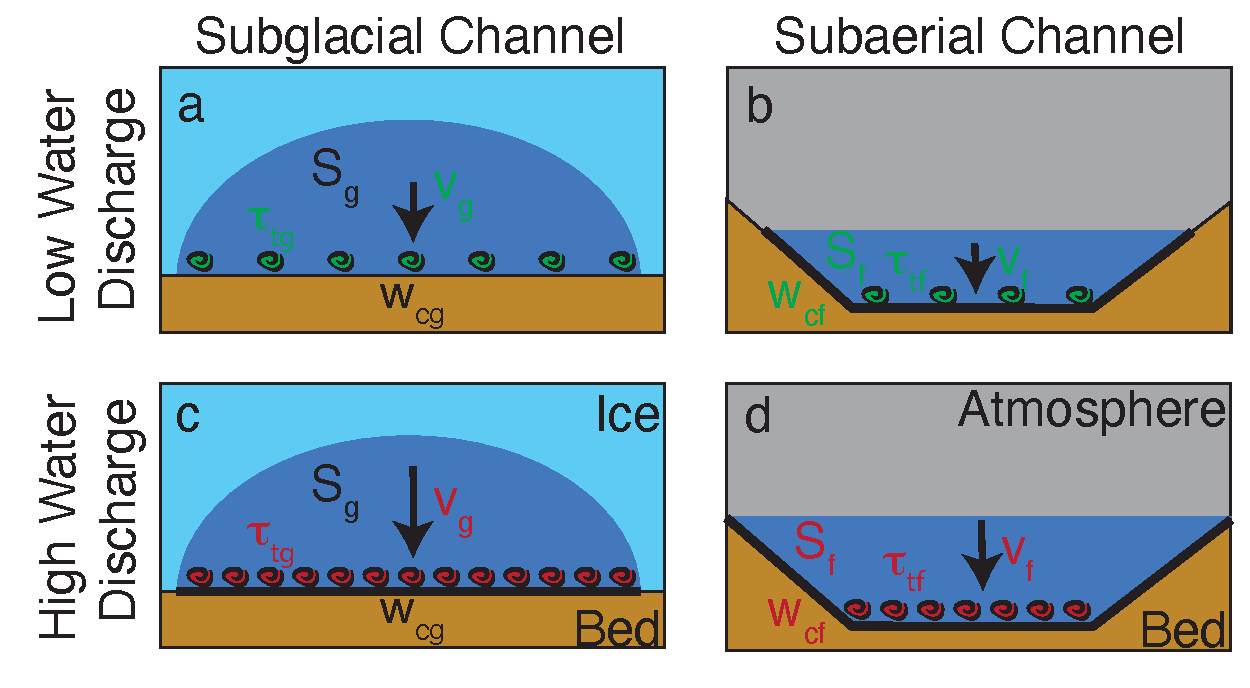
\includegraphics[width=0.8\linewidth]{Fig1.pdf}
    \caption{Sketch for the different responses of subglacial and subaerial channels to increased water discharge over short time-scales.
      Arrow length denotes water velocity magnitudes in the subglacial (subaerial) $v_g$ ($v_f$) channels.
      $S_g$ ($S_f$) represents the wetted area in subglacial (subaerial) channels.
      The subglacial channel width $w_g$ remains unchanged, while the subaerial channel width $w_f$ evolves with water discharge.
      Subglacial (subaerial) shear stress $\tau_g$ ($\tau_f$) is responsible for the mobilization of sediment.
    }
    \label{fig:cartoon}
  \end{figure}

Because of the above, sediment mobilization in subaerial and subglacial channels responds differently to changing water discharge.
These differences are implicitly included in a wide range of available models that  quantify sediment transport in both subglacial and subaerial channels  \cite<e.g.>{walder1994,alley1997,tucker1997,creyts2013,delaney2019,hewitt2019,wickert2019}.
The divergent response of changing water discharge on sediment mobilization capacity may well impact sediment dynamics near glacier margins where flow transitions from pressurized to open channel flow \cite<e.g.>{perolo2018}.
Additionally, the variable response of sediment transport capacity to water discharge in the two systems may affect the interpretation of sediment transport records in glacial systems \cite<e.g.>{muller1968,richards2003,swift2005,ganti2016}.
Yet, little work has examined the differing relationship between variations in water discharge and sediment discharge in subglacial and subaerial channels \cite{alley1997}.

This manuscript evaluates the relationship between sediment transport capacity and water discharge in subglacial channels and compares it to subaerial ones.
Models of subglacial and subaerial hydraulics are used to quantify the respective water velocity and channel morphology.
The models are applied to hydrological records from an Alpine glacier in Switzerland (Fieschergletscher) and  a land-terminating glacier in Greenland (Leverett Glacier).
The  lumped nature of the models isolates the disparity between water discharge and sediment transport capacity in subglacial systems, independent of the upstream drainage network and sediment access.
Outputs demonstrate differences in the relationships between  water discharge, channel geometry, and water velocity in the subglacial and subaerial channels.
The manuscript then uses the demonstrated differences between the two channel types to discuss the implications for interpreting the processes driving variability in sediment transport records and their relationship with hydrology from glacierized catchments.

\section{Study sites and data}
\label{sect:ss_data}

Water discharge data is used from Alpine and ice sheet settings collected downstream of the glacier, assuming no water storage in the proglacial area.
The Alpine site (labeled \alpine{}) is  Fieschergletscher in the Swiss Alps ($46^\circ\,29'\,07''$ N, $8^\circ\,08'\,3''$ E).
The water discharge data used here was collected at a $1$\unit{min} interval from May 24, 2014, to October 10, 2014 \cite{felix2021,felix2022}.

The Leverett Glacier in Greenland (labeled \icesheet{}) serves as the ice sheet setting.
Water discharge was collected roughly $2$\unit{km} downstream from the terminus between June and August/September 2009 to 2012 ($67^\circ\,03'\,5''$ N, $50^\circ\,12'\,59''$ W).
Data is used in \citeA{tedstone2017} and \citeA{hawkings2014} at a $5$\,\unit{min} time interval from May 28, 2012 to August 8, 2012.

Note that sediment discharge records are omitted from the analysis here given the role of sediment supply, in addition to capacity, on capturing variations in sediment discharge \cite<e.g.>{delaney2024}.

\section{Methods}
\label{sect:meth}
The models described below (Sections ~\ref{sect:sub_mode}~and~\ref{sect:fluv}) represent relationships amongst water discharge, water velocity, and channel geometry in both subaerial and subglacial channels (Table \ref{table:vpm}).
Both models use the measured discharge to calculate water velocity, shear stress, and width-integrated shear stress, upon which both suspended sediment and bedload transport depend \cite<Figure \ref{fig:cartoon}; >{shields1936}.
The evaluation of these variables omits the selection of a sediment transport relationship and a grain-size parameter \cite<e.g.>{shields1936,meyer1948}.


\subsection{Subglacial channel  model}
\label{sect:sub_mode}

To evaluate the shear stress of water flowing across sediments underneath a glacier, the subglacial channel model accounts for the channel geometry and the velocity of the flowing water.
To do this, we use a lumped hydraulics model from \citeA{werder2010b}, itself based upon  \citeA{clarke1996}.

Here, it is assumed that the water is transported through a subglacial channel \cite<Figure~\ref{fig:cartoon}; >{rothlisberger1972} beneath a glacier with channel length $l$, with a flatbed and a mean thickness of $h_{ice}$.
The channel  size grows from melt due to frictional heating from water flow and closes due to the creep  of the ice.
The formulation here does not consider the englacial storage of water.
The evolution of subglacial channel size $S_g$ is given as
\begin{linenomath*}
  \begin{equation}
    \label{eq:dS_dt}
    \frac{\partial S_g}{\partial t} = C_1 \frac{Q \Delta h}{l} - C_2 \left(h_{o}-\frac{\Delta h}{2}\right)^n\,S_g,
  \end{equation}
\end{linenomath*}
\noindent where $t$ is time, $C_1= (1-\rho_wc_pc_t)\,\frac{\rho_wg}{\rho_iL}$ and $C_2=2A(\frac{\rho_wg}{n})^n$ are constants (complete values given in Table \ref{table:vpm}), $g$ is the acceleration due to gravity, $Q$ is water discharge, $\Delta h$ is the hydraulic potential change over $l$, $h_{o}= \frac{\rho_i}{\rho_w} h_{ice}$ is the mean ice overburden pressure expressed in meter water equivalent ($\rho_w$ is density of water; $\rho_i$ is density of ice), and $n$ is Glen's n \cite{glen1955} (usually $n=3$).
The first term on the right side of the equation represents the opening of the channel through frictional heating, while the following term represents the creep closure of the channel from ice deformation.


Following the Darcy-Weisbach equation, the head drop $\Delta h$ is
\begin{linenomath*}
  \begin{equation}
    \label{eq:dh}
    \Delta h \,  = l \,\frac{1}{2g} \,f_r\,\frac{v_g^2}{D_h},
  \end{equation}
\end{linenomath*}
\noindent where $f_r$ is a friction factor, $D_h$ is the hydraulic diameter, $l$ is the channel length, and $v_g=\frac{Q}{S_g}$ is the water flow speed.
%
The hydraulic diameter $D_h$ is converted to wetted area $S_g$ with
\begin{equation}
  \label{eq:Dh2S}
  S_g= \frac{D_h^2}{2}\,\frac{(\frac{\beta}{2}+\sin \frac{\beta}{2})^2}{\beta - \sin \beta},
\end{equation}
where $\beta$ is the central angle of the circular segment that comprises the channel (the so-called Hooke angle, \citeA{hooke1990}). Note that $\beta =\pi$ corresponds to a semi-circular channel and smaller values of $\beta$ result in shallow, wide channels.
This completes the subglacial hydraulic model which is described by the state variables $S_g$ and $\Delta h$.

The shear stress, $\tau_g$, between the water and the channel bed is determined through the Darcy-Weisbach formulation
\begin{equation}
  \label{eq:tau_g}
  \tau_g=\frac{1}{8}\,f_r\,\rho_w\,v_g^2,
\end{equation}
%
where $v_g = \frac{Q}{S_g}$ is the water velocity.
%
The width of the channel floor $w_g$ is represented as
\begin{equation}
  \label{eq:dh2wc}
  w_g = 2  \sin \frac{\beta}{2} \sqrt{\frac{2\, S_g}{\beta -\sin \beta}}.
\end{equation}
%
This value is used to establish the integrated shear stress across the channel $w_g\tau_g$.

\subsection{Subaerial channel  model}
\label{sect:fluv}

% To parameterize the shear stress of water flowing across sediments in the subaerial channel, the hydraulics parameterization presented in \citeA{tucker1997} is implemented.
Using mass conservation and the Darcy-Weisbach relationship as well as assuming that the channel is sufficiently wide compared to its depth so that the hydraulic radius is well approximated by the flow depth,
the shear stress $\tau_f$ at the river bed is
\begin{linenomath*}
  \begin{equation}
    \label{eq:DW_tau}
    \tau_f=\frac{\rho_w\,g^{\frac{2}{3}}\,f_f^{\frac{1}{3}}}{2}\, \Big(\frac{Q}{w_f} \Big)^{\frac{2}{3}} \,\nabla z_c^{\frac{2}{3}},
  \end{equation}
\end{linenomath*}
where $\nabla z_c$ is the channel slope, and $f_f$ is the friction factor for subaerial channels \cite{tucker1997}.
Channel width $w_f$ is
\begin{equation}
  \label{eq:wcf}
  w_f = k \, Q^{\alpha},
\end{equation}
%
where $k$ is a constant and $\alpha=\frac{1}{2}$ is a commonly chosen exponent \cite{leopold1953}.
Also following the Darcy-Weisbach, subaerial water velocity, $v_f$, is given as
\begin{equation}
  \label{eq:vf}
  v_f = \sqrt{\frac{8\,\tau_f}{f_f\,\rho_w}}.
\end{equation}
%
As above, the width-integrated shear stress is $w_f\tau_f$.

Note that this subaerial channel model is purely algebraic, whereas the subglacial model comprises a differential equation for the evolution of $S_g$.
Thus the channel size in the subaerial model has no history dependence on the discharge $Q_w$, where as the subglacial one does (Equation~\ref{eq:dS_dt}).

\subsection{Implementation}
\label{sect:imp}

The models above are applied to proglacial discharge records from the Fieschergletscher (scenario \alpine{}) and the Leverett Glacier (scenario \icesheet{}), using subglacial model outputs that are contrasted with subaerial ones.
Outputs of the models represent generalizable sediment transport characteristics from these hydrographs, rather than actual hydraulic conditions.
To generalize these scenarios, \alpine{}  is exemplified by Fieschergletscher's relatively thin ice thickness \cite<$h_{ice}$: $225$\,\unit{m}>{grab2021}, low water discharge ($\sim\,10$\,\unit{m}$^3$\,\unit{s}$^{-1}$) and high diurnal variability in water discharge (Figure~\ref{fig:model_outs}, a).
\icesheet{}  is exemplified by Leverett glacier's  thick ice  \cite<$h_{ice}$: $700$\,\unit{m}; >{morlighem2017}, high water discharge \cite<$\sim\,300$\,\unit{m}$^3$\,\unit{s}$^{-1}$>{tedstone2017}  and low diurnal variability in water discharge (Figure~\ref{fig:model_outs}, e).
%However, both scenarios share a discharge with a similar, relative seasonal amplitude.

In the first experiment, the models are  applied to a reference test case for each glacier that assumes  a subglacial channel with $\beta=\frac{\pi}{6}$%, i.e. a segment of a quarter-circle,
(Table~\ref{table:vpm}).
Both friction factors $f_r$ and $f_f$ are tuned so that reasonable water velocities \cite<$\sim\,1.6\,$\unit{m}\,\unit{s}$^{-1}$>{werder2010b,chandler2013} occur for both \alpine{} and \icesheet{}.
The initial condition of cross-sectional area $S_g$ is evaluated by applying a model spinup with the maximum observed water discharge for the first $4$ days of the study until there is no change in channel area. 
The subaerial channels of both scenarios have a bed slope of $\nabla z_c = 0.05$ (Table~\ref{table:vpm}).

The results below present water velocity ($v_g$, $v_f$), shear stress ($\tau_g$, $\tau_f$), and width-integrated shear stress ($w_g\tau_g$, $w_f\tau_f$) from the subglacial and subaerial models.
For brevity, these values together are referred to as ``model outputs'' in the text.
To quantify the link between sediment transport capacity and water discharge, model outputs are compared to water discharge from the glaciers using Spearman rank correlation, which varies with the ordering of values.
Rank correlation reduces the impact of the non-linear response of sediment transport capacity to the hydrological forcing.

A second experiment aims to further characterize the variability in sediment discharge capacity in subglacial compared to subaerial channels across a range of channel shapes, friction factors, and water discharge variability. 
To accomplish this, we examine the variability of one model output (i.e water velocity) by evaluating its standard deviation throughout the season.

The effect of channel shape and roughness is established by running the model with random parameter values of channel geometry factors ($\beta$ and $k$) and friction factors ($f_r$ and $f_f$; see Table~\ref{table:vpm} for value range).
Runs with parameter combinations are accepted if their mean subglacial water velocity over the season lies between $0.75$\,\unit{m}\,\unit{s}$^{-1}$ and $2$\,\unit{m}\,\unit{s}$^{-1}$ or if subaerial water velocity lies between $0.3$\,\unit{m}\,\unit{s}$^{-1}$ and $1.2$\,\unit{m}\,\unit{s}$^{-1}$, following measurements \cite<e.g.>{werder2010b,magnusson2012,chandler2013}.
Additionally, to be accepted, model runs can only experience a flotation fraction ($\frac{\Delta h}{2\,h_o}$) of above $1.2$ for less than $2.5$\,\% of the run.

The routine runs until $100$ different parameter combinations for each water discharge aggregation period are accepted with the conditions described above.
Here, the water discharge input at a given time is the average over the aggregation period before that time, ranging from $15$\,\unit{min} up to $15$\,\unit{days}.




\section{Results}
\begin{figure}[h]
  \centering
  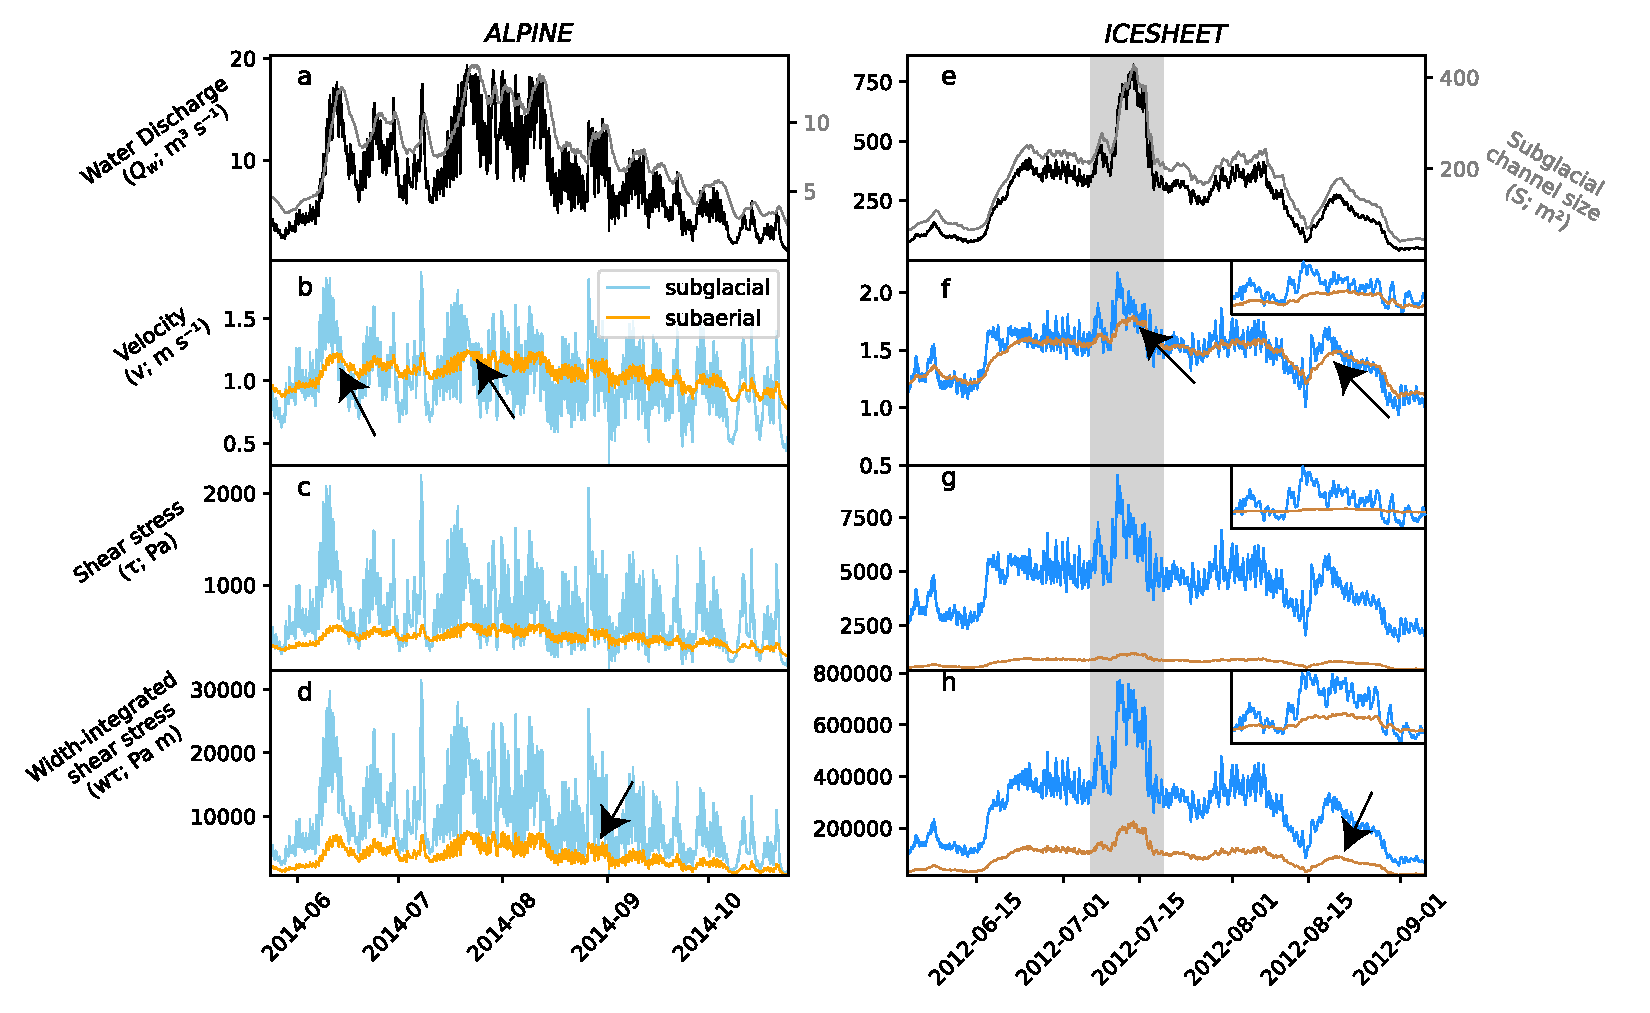
\includegraphics[width=0.9\linewidth]{Fig2.pdf}
  \caption{Model outputs from simulations using the hydrographs in panels a and e for the scenarios \alpine{} (a-d) and \icesheet{} (e-h).
    Gray (black) lines in a and e represent the subglacial channel size (water discharge).
    Blue (orange) lines represent outputs from the subglacial (subaerial) channel.
    Data are shown at $15$\unit{min} intervals.
    Arrows denote where variables peak in the subglacial channel before the subaerial one.
    Insets in f-h show the  peak melt event denoted by the shaded area in panels e--h, but have arbitrary y-axis.
    % Note that the x and y axes are different for \alpine{} and \icesheet{}.
  }
  \label{fig:model_outs}
\end{figure}

Following the first experiment defined in Sections~\ref{sect:imp}, model outputs exhibit different seasonal evolutions and peaks.
Water velocity and shear stress represent the potential for sediment mobilization, and width-integrated shear stress represents a proxy for the total sediment transport capacity across the channel bed (Figure~\ref{fig:model_outs}).
Furthermore, the subglacial model outputs are generally larger than their subaerial equivalents, thus greater sediment transport capacity would be expected in subglacial channels compared to subaerial ones.

\begin{figure}[h]
  \centering
  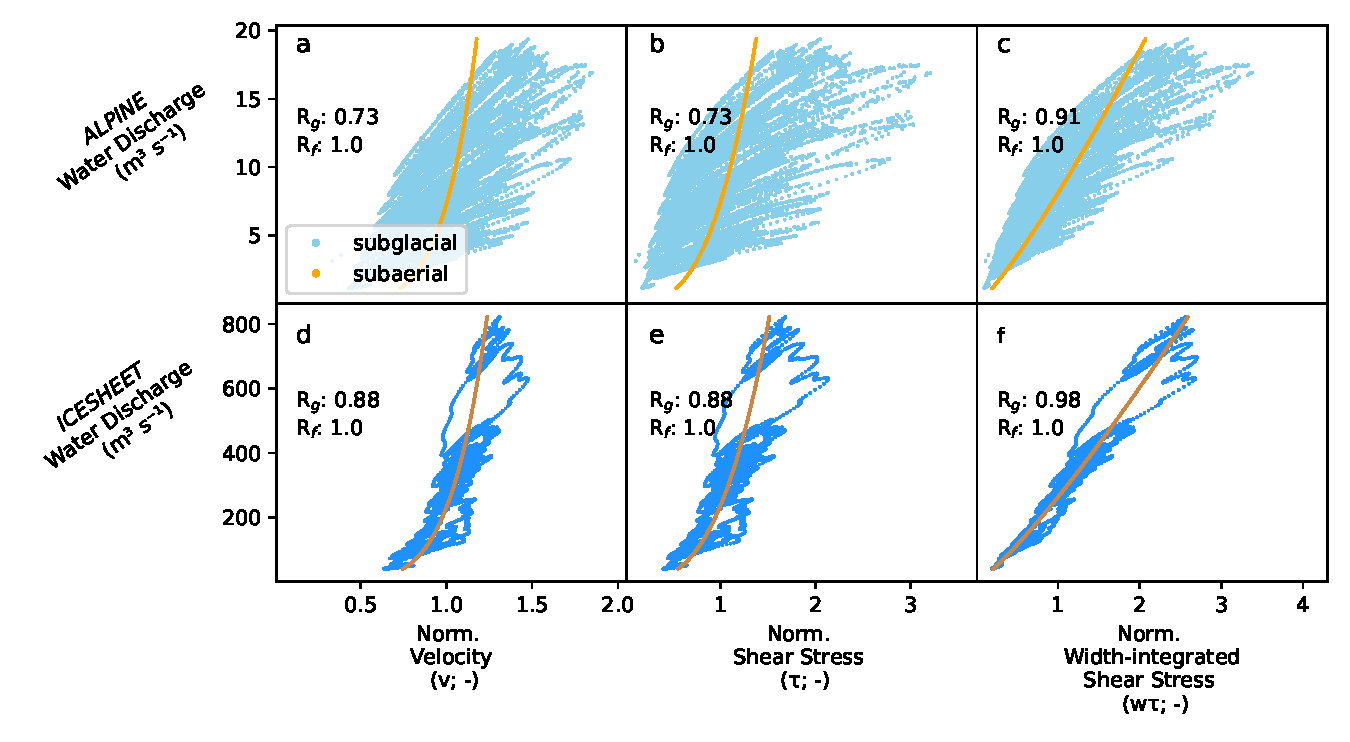
\includegraphics[width=0.9\linewidth]{Fig3.pdf}
  \caption{
    Relationship between water discharge and normalized velocity, shear stress, and width-integrated shear stress for \alpine{} (a-c) and \icesheet{} (d-f).
    Variables on the x-axis have been normalized to mean values.
    $R_g$ ($R_f$) shows the Spearman rank correlations for the subglacial (subaerial) outputs.
    Plots are shown with discharge and outputs at $15$\unit{min} intervals.
  }
  \label{fig:Qw_vari}
\end{figure}

Examining the relationship between water discharge and the model outputs, a different relationships emerge between the subaerial and subglacial cases, due to the hysteresis in channel size in the subglacial model (Equation~\ref{eq:dS_dt}).
Because there is no history dependence in  subaerial channels, each water discharge value in the subaerial channel results in a unique water velocity, shear stress, and width-integrated shear stress (Section~\ref{sect:sub_mode}).
This characteristic results in a perfect rank correlation between the variables (Figure~\ref{fig:Qw_vari}).

Conversely, the history dependence on channel size in subglacial channels means different outputs occur across a range of discharges.
For instance, in subglacial channels in \alpine{}, very high seasonal water velocity values and shear stresses can occur from a low water discharge  ($\sim\,4$\,\unit{m}$^3$\,\unit{s}$^{-1}$) to the maximum water discharge at over ($17$ \,\unit{m}$^3$\,\unit{s}$^{-1}$, Figure~\ref{fig:Qw_vari}\,a).
In \icesheet{}, water velocities close to the seasonal mean value can occur at water discharges between roughly $150$ \,\unit{m}$^3$\,\unit{s}$^{-1}$ and $310$ \,\unit{m}$^3$\,\unit{s}$^{-1}$.
When considering the subglacial channel's evolving width, width-integrated shear stress  across the channel generally increases with water discharge, with improved rank correlation compared to water velocity or shear stress (\alpine{}, Figure~\ref{fig:Qw_vari} a--c).
Yet even the width-integrated shear stress  can vary substantially, with the highest values occurring at water discharge values ranging from roughly $11$ \,\unit{m}\,\unit{s}$^{-1}$ to over $17$ \,\unit{m}\,\unit{s}$^{-1}$.
The variability in width-integrated shear stress is less pronounced in the \icesheet{} scenario, where the hydrograph has less diurnal variability (Figure~\ref{fig:Qw_vari} c, f).

The different response of subaerial and subglacial model outputs to water discharge impacts the timing of peaks in sediment transport capacity.
In the subglacial channel, peaks in $w_g\tau_g$ generally occur when water discharge increases at the fastest rate, but before the maximum water discharge (Figure~\ref{fig:model_outs}\, d and h).
By contrast, in the subaerial channel,   $w_f\tau_f$  peaks when water discharge is highest.

\begin{figure}[h]
  \centering
    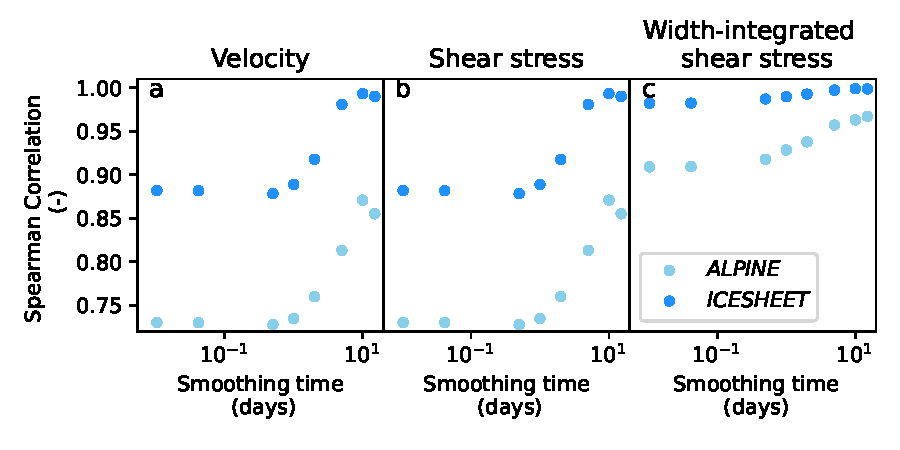
\includegraphics[width=0.9\linewidth]{Fig4.pdf}
    \caption{Standard deviation of model outputs for different time aggregations with different subglacial and subaerial channel shapes and friction factors.
      Shaded areas denote the range of results from the accepted $100$ parameter combinations (Section~\ref{sect:imp}).
      Solid lines denote  mean values.
      Markers show aggregation periods ($15$\,\unit{min}, $1$\,\unit{hr}, $12$\,\unit{hr}, $1$\,\unit{d}, $5$\,\unit{d}, $10$\,\unit{d}, and $15$\,\unit{d}).
       }
    \label{fig:multi_run}
  \end{figure}

The second numerical experiment aims to evaluate the role of channel shape and friction factors on the findings above and to examine the effect of variability in water discharge.
Across the range of channel shapes and friction factors  examined (Section\,\ref{sect:imp}), variability in water velocity and shear stress remains higher in the subglacial system compared to the subaerial one in both \alpine{} and \icesheet{}.
This suggests that there is greater intermittency and variability in sediment transport in subglacial systems compared to subaerial ones, especially in supply-limited systems where sediment could be exhausted or mobilized over diurnal discharge cycles.
In contrast, in \alpine{}, the variability in width-integrated shear stress is comparable between the subaerial and subglacial systems, due to the highly variable water discharge, largely due to diurnal variations (Figure~\ref{fig:multi_run}).
However, in \icesheet{}, with lower water discharge fluctuations, the variability in width-integrated shear stress remains consistently higher in the subglacial system across the time aggregation periods.

Results from  both \alpine{} and \icesheet{} scenarios show that the variability in subglacial  decreases with aggregations longer than approximately 1--5 days (Figure~\ref{fig:multi_run}).
Yet, substantial differences in the variability between the model outputs for subglacial and subaerial cases persist in periods of up to $15$ days, longer than which seasonal variations might be conflated.
Note that the timing of peak sediment transport conditions still occurs, across these periods, and they are are thus not captured in aggregating water discharge over longer periods (Figure~\ref{fig:model_outs}).

\section{Discussion}

\subsection{Hydrology and evolving channel shape in driving sediment transport variability}
\label{sect:dis_qsc}

Model outputs (water velocity, shear stress, and width-integrated shear stress) vary differently in response to water discharge in subglacial channels compared to subaerial ones (Figure~\ref{fig:Qw_vari}).
In sediment transport relationships that evaluate sediment discharge capacity, such as in \citeA{meyer1948} or \citeA{engelund1967}, shear stress is scaled to the power of $\frac{3}{2}$ or $\frac{5}{2}$, respectively.
The exponent greater than $1$ magnifies sediment discharge variability beyond the variable sediment transport parameters described above (Figure~\ref{fig:multi_run}; Table~\ref{tab:Qs}).

Sediment transport capacity in subglacial channels responds more rapidly to changes in water discharge compared to their subaerial counterparts \cite<Figures~\ref{fig:Qw_vari}~and~\ref{fig:multi_run}>{alley1997}.
In subglacial R\"othlisberger channels in steady state with water discharge, the width-integrated shear stress response to water discharge is $ w_g\,\tau_{g}\, \propto\,  Q^{\sim\frac{4}{5}}$ (Table\,\ref{tab:eqs1}).
However, subglacial channels rarely operate in a steady state \cite<e.g.>{gimbert2016}.
For sufficiently short periods, channel width and wetted area are fixed in the subglacial system (akin to pipe flow) so that the response of width-integrated shear stress is $w_g\, \tau_{g}\, \propto\,  Q^{2}$ (Table\,\ref{tab:eqs1}).
\ref{sect:scaling} provides a complete description of sediment transport capacity in different drainage conditions.
Note that in pipe flow conditions, maximum sediment transport would coincide with peak water discharge and a co-varying relationship with water discharge would occur, unlike with the evolving channel size here where a disparate relationship with water discharge occurs (Section~\ref{sect:sub_mode}; Figure \ref{fig:model_outs} and \ref{fig:Qw_vari}). 
Similar adjustments in channel shape occur in subaerial channels \cite{phillips2016}, albeit at timescales longer than the subglacial channel's response time of hours to days.

Substantial differences emerge in model outputs between the different hydrological forcings of the \alpine{} and \icesheet{} cases.
Indeed, the more decoupled and sporadic relationship between model outputs and water discharge in \alpine{} results from the
relatively larger discharge variations on daily to weekly timescales compared to \icesheet{}.
This occurs as the evolution of the R-channel's size is small compared to the variations in water discharge.
Such water discharge variability in alpine catchments may cause shear stress to approach the water discharge squared \cite< \ref{sect:scaling}; c.f.>{alley1997}.
With respect to \icesheet{}, a closer approximation of the hydraulics could be represented by pipe flow here, where the channel size remains fixed.
Conversely, the reduced variability in water discharge in \icesheet{} may result in the R-channel's size being closer to equilibrium concerning the variations in water discharge.
In this case, the exponent on water discharge for shear stress is likely less than $2$, but greater than $\frac{4}{5}$ occurring when the R-channel's size evolves in equilibrium with water discharge (see \ref{sect:scaling}).
As a result, a stronger correlation persists between subglacial model outputs and water discharge in \icesheet{} compared to \alpine{} (Figure~\ref{fig:Qw_vari}).


\subsection{Effect sediment transport and landscape evolution}

The stronger link between sediment transport capacity and water discharge in subaerial channels may mean that variations in sediment transport records can be more easily attributed to hydro-climatic conditions than in subglacial systems.
A glacier's sediment transport capacity is impacted by the ice thickness controlling the channel closure rate, and the glacier's surface slope, in addition to water discharge and sediment size \cite<Figure~\ref{fig:multi_run}, Section~\ref{sect:sub_mode}; >{rothlisberger1972,shreve1972,gimbert2016,stevens2022,walder1994}.
In a supply-limited state, the glaciers' sediment discharge record also responds to  sediment availability and bedrock erosion from  water pressure variations and sliding  \cite<e.g.>{iverson2012,herman2015,delaney2023}.
This multitude of processes lies in contrast to many subaerial channels, where transport capacity typically responds to sediment size, channel shape, water discharge, and hydraulic gradient.
The hydraulic gradient and channel shape can remain stable over years to millennia \cite<Section~\ref{sect:fluv}; e.g.>{tucker1997,wickert2019}.

Previous work suggests that this co-varying relationship between sediment discharge capacity in  subaerial conditions could be noticeable $\sim20$\,\unit{km} downstream of the Leverett site, where a strong correlation persists between sediment plume size and the river's water discharge into the Kangerlussuaq fjord \cite{mcgrath2010}.
In contrast, in marine-terminating glacier catchments, a less consistent relationship may occur between water discharge or melt extent and sediment plume size \cite{tedstone2012}.
Here, ocean water pressurizes subglacial channels at the ice front \cite<e.g.>{how2017}, so the reduced correlation could result from the inconsistent relationship between subglacial sediment transport capacity and water discharge presented here.

Furthermore, the greater variations in subglacial sediment transport capacity compared to subaerial ones could cause a supply-limited regime to persist at many glaciers.
In subglacial systems, sediment's critical shear stress, or threshold at which sediment mobilization occurs, can be reached more frequently and across a range of water discharges, compared to subaerial systems (Figure~\ref{fig:Qw_vari}).
Sediment exhaustion through this process may  explain the stronger dependence of sediment discharge from the Greenland Ice Sheet on basal shear stress, a proxy for bedrock erosion, rather than glacier melt \cite{overeem2017}.

\subsection{Parameterizing  sediment transport in glacierized catchments}

Numerical models of subglacial sediment transport generally apply classical parameterizations of subglacial hydrology to evaluating sediment transport conditions \cite<e.g>{hewitt2019,beaud2018}.
In these R-channel models, realistic water pressure regimes can be achieved by changing the channels shape and friction factor, therefore  model tuning is done with the friction factor and leaving the channel shape fixed as a semi-circle \cite<$\beta =\pi$; >{werder2010b}.
However, the role of channel width in the findings here suggests that more thorough parameterization of channel shape and channel width is needed in assessing subglacial sediment transport capacity as compared to water pressure (Section\,\ref{sect:sub_mode}, \ref{sect:scaling}).

Water discharge measurements at the hourly timescale remain unavailable in many catchments, further limiting the ability of subglacial  sediment transport models to capture certain events.
The model outputs' variability in subglacial channels approaches that of subaerial ones over $1-5$ days of  aggregation (Figure~\ref{fig:multi_run}), possibly resulting in parity in sediment transport capacity variations between subaerial and subglacial channels over these periods.
Note that although variability between the events could remain comparable, water discharge forcings aggregated over periods longer than days may omit key sediment discharge characteristics, such as the timing of peaks in sediment transport capacity from glaciers (Figure~\ref{fig:model_outs}).


\section{Conclusions}

The sediment transport capacity of a channel is driven by its width and the shear stress exerted by the flowing water, which is proportional to the square of the flow velocity.
Subaerial channels alter both their channel width and water velocity immediately in response to changing water discharge.
In contrast, pressurized subglacial channels largely accommodate rapidly changing water discharge by altering water velocity.
Their size responds over several days to changes in discharge.
Thus the response of sediment transport capacity is much more sensitive to changes in water discharge in subglacial channels compared to subaerial ones.

Implications of the presented findings include:
\begin{enumerate}
\item the changing relationship between water discharge and sediment transport capacity below glaciers creates larger variability in sediment transport capacity compared to river systems;
  \vspace{.1cm}
 
\item
  water discharge variability impacts subglacial sediment transport capacity fluctuations to a larger degree than subaerial channels;
  \vspace{.1cm}
  
\item the uneven response of sediment transport capacity to water discharge variations shows a different response and timing to periods of elevated water discharge in subglacial channels compared to subaerial ones.
However, representing subglacial sediment transport capacity with either open-channel flow or pipe flow neglects differences in timing.
\end{enumerate}

This study calls for the careful analysis of the relationship between sediment transport capacity and water discharge when examining sediment discharge from glacierized catchments.

\section*{Author Contributions}

I.D. designed the study, developed, and implemented the model and experiments, and wrote the manuscript.
A.J.T. helped interpret data from Leverett Glacier and provided guidance on experiment design.
M.A.W. provided data from Fieschergletscher and added the relationship between shear stress and water discharge (see \ref{sect:scaling}).
D.F. provided data from Fieschergletscher.
All authors provided key inputs in writing and editing the manuscript.


\section*{Open Research Section}

Code to make the figures, with links to the data, can be found at \url{https://bitbucket.org/IanDelaney/xsection/src/master/}.
Code and data will be uploaded to a permanent repository, with FAIR principles, pending acceptance of the paper.

\acknowledgments

SNSF Project No. $\mathrm{PZ00P2}$\_$202024$ provided  funding for I. Delaney.
A. Tedstone acknowledges funding from the European Research Council, award $818994$ -- CASSANDRA.
G. King and M. J. Gevers provided useful comments on a previous version of this manuscript.

\bibliography{PaperLib}

\newpage

\appendix

\section{Table of variables, parameters and constants}
\begin{table}[h]
  \centering
  \caption{Variables, parameters, and constants used in this work.
    Where two values are given, the first refers to  \alpine{}, a scenario from Fieschergletscher, and the second to a glacier marginal to the \icesheet{} a scenario from Leverett Glacier. If a second line is given, it refers to the range of values examined in the parameter search}
  \small % TODO remove again
  \begin{tabular}{ l  c  c c }
    Name &Symbol&  Value&Units \\
    && (\alpine{} or \icesheet{})\\
    \hline
    \textbf{Variables}  & & & \\
    Water discharge  & $Q$& & $\mathrm{m^{3}\,s^{-1}}$ \\
    Water velocity (subglacial, subaerial)  & $v$, ($v_g,\,v_{f}$)& & $\mathrm{m\,s^{-1}}$ \\
    Channel wetted area (subglacial, subaerial) &  $S_g, S_f$& & $\mathrm{m^2}$     \\
    Channel depth (subaerial) & $H$&& $\mathrm{m}$\\
    Hydraulic diameter &$D_h$&&$\mathrm{m}$\\
    Width of channel floor (subglacial, subaerial) & $w$, ($w_g,w_f$)&  & $\mathrm{m}$     \\
    Hydraulic head &$\Delta h$&& $\mathrm{m}$\\
    Hydraulic gradient &$\Psi=\frac{\Delta h}{l}$&& $\mathrm{m\, m^{-1}}$\\
    Shear stress (subglacial, subaerial) & $\tau$, ($\tau_g,\,\tau_f$) && $\mathrm{Pa \, m^{-2}}$ \\
    Stream power & $\Omega$ && $\mathrm{ kg \, m\, s^{-3}}$ \\

         &&&\\

    \textbf{Parameters and Constants}  & & &\\
    Gravitational constant&$g$& $9.81$&$\mathrm{m\,s^{-2}}$\\
    Density of water & $\rho_w$& $1000$ & $\mathrm{kg\,m^{-3}}$ \\
    Density of ice & $\rho_i$& $900$ & $\mathrm{kg\,m^{-3}}$ \\
    Hooke angle of channel & $\beta$ & $\frac{\pi}{6}$ & \unit{rad}\\
         && ($\frac{\pi}{10}$, $\pi$) & \\
    Friction factor (subglacial, subaerial) & $f$, ($f_r$, $f_f$) &$5$ or $16$, $3$ & $\mathrm{(-)}$ \\
         && ($0.01$, $21$) & \\
    Glacier thickness &$h_{ice}$& $225$ or $740$  &\unit{m}\\
    Effective glacier thickness &$h_o$&$\frac{\rho_i}{\rho_w} h_{ice}$  &\unit{m}\\
    Effective glacier length &$l$& $7,000$ or $26,000$&\unit{m}\\
    Constant $1$ in Equation~\ref{eq:dS_dt} &$C_1$&$2.2\times10^{-5}$&\unit{m}$^{-1}$\\
    Constant $2$ in Equation~\ref{eq:dS_dt} &$C_2$&$3.7\times10^{-13}$&\unit{m}$^{-n}\,s^{-1}$\\
    Latent heat of fusion &$L$&$333.5 $&\unit{kJ\,kg}$^{-1}$\\
    Pressure melting coefficient &$c_t$&$7.5\times 10^{-8}$&\unit{K\,Pa}$^{-1}$\\
    Specific heat capacity of water &$c_p$&$4180$&\unit{J\,kg}$^{-1}$\unit{K}$^{-1}$\\
    Ice flow constant &$A$& $5.3\times10^{-24}$ &\unit{Pa}$^{-n}$\,$s^{-1}$\\
    Ice flow exponent &$n$& $3$ &$\mathrm{(-)}$\\
   
    Gradient of channel bed (subaerial) &$\nabla z_c$ &$0.05$& $\mathrm{(-)}$\\
    Subaerial channel factor & $k$ &$3$ or $6.5$ & $\mathrm{s\,m^{-2}}$\\
     && ($5$, $20$) & \\
    Channel geometry exponent &$\alpha$& $\frac{1}{2}$&$\mathrm{(-)}$ \\
    \hline
  \end{tabular}
  \label{table:vpm}
\end{table}
\FloatBarrier

\section{Figure 3 over various time aggregations}

\begin{center}
  \begin{figure}[!h]
    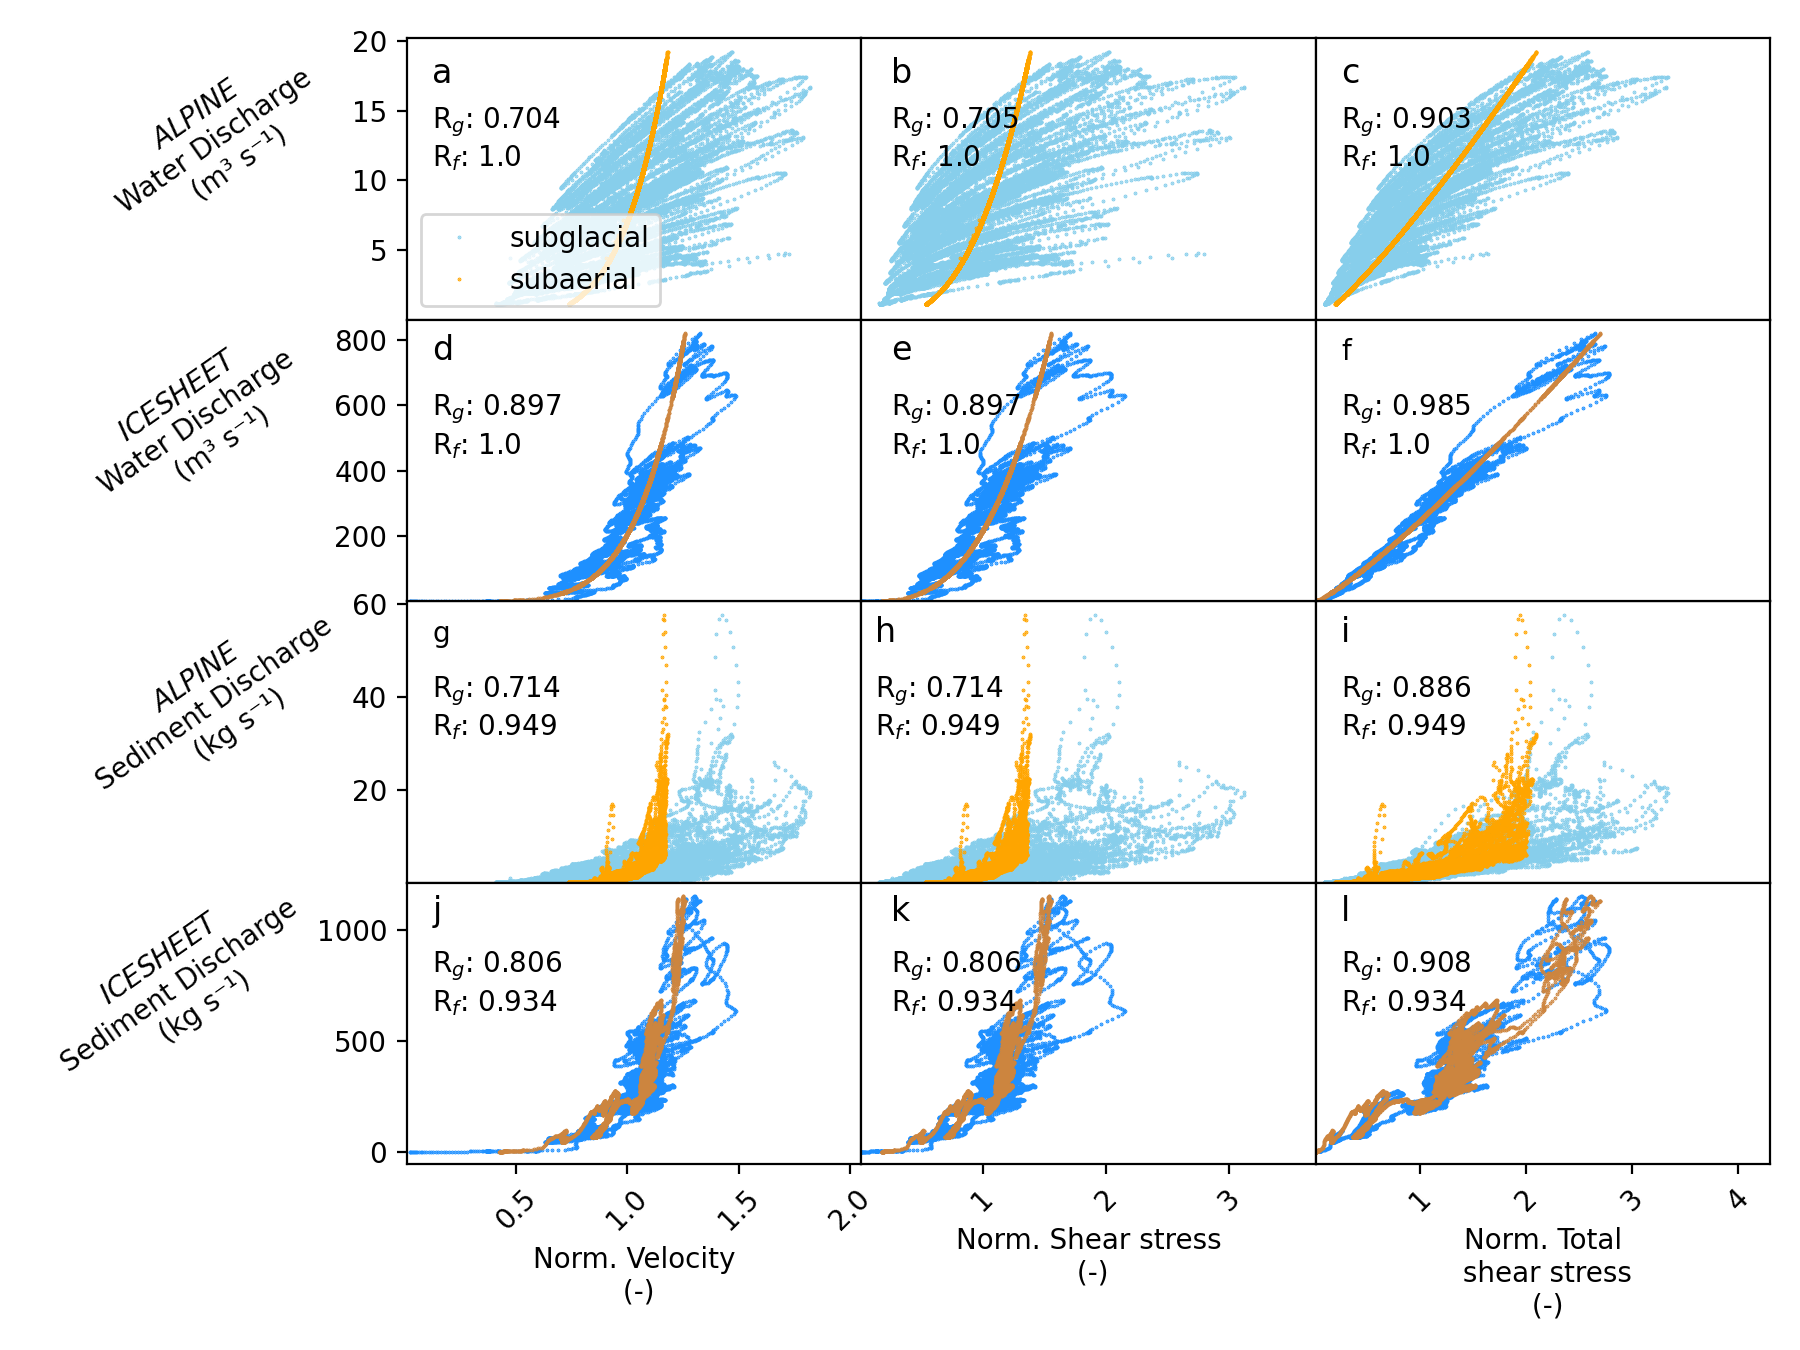
\includegraphics[width=0.7\linewidth]{Fig3_hr.png}
    \caption{As Figure \ref{fig:model_outs}, with $1$ \,\unit{hr} aggregation.}
    \label{fig:model_outs_1hr}
  \end{figure}
\end{center}

\begin{center}
  \begin{figure}[!h]
    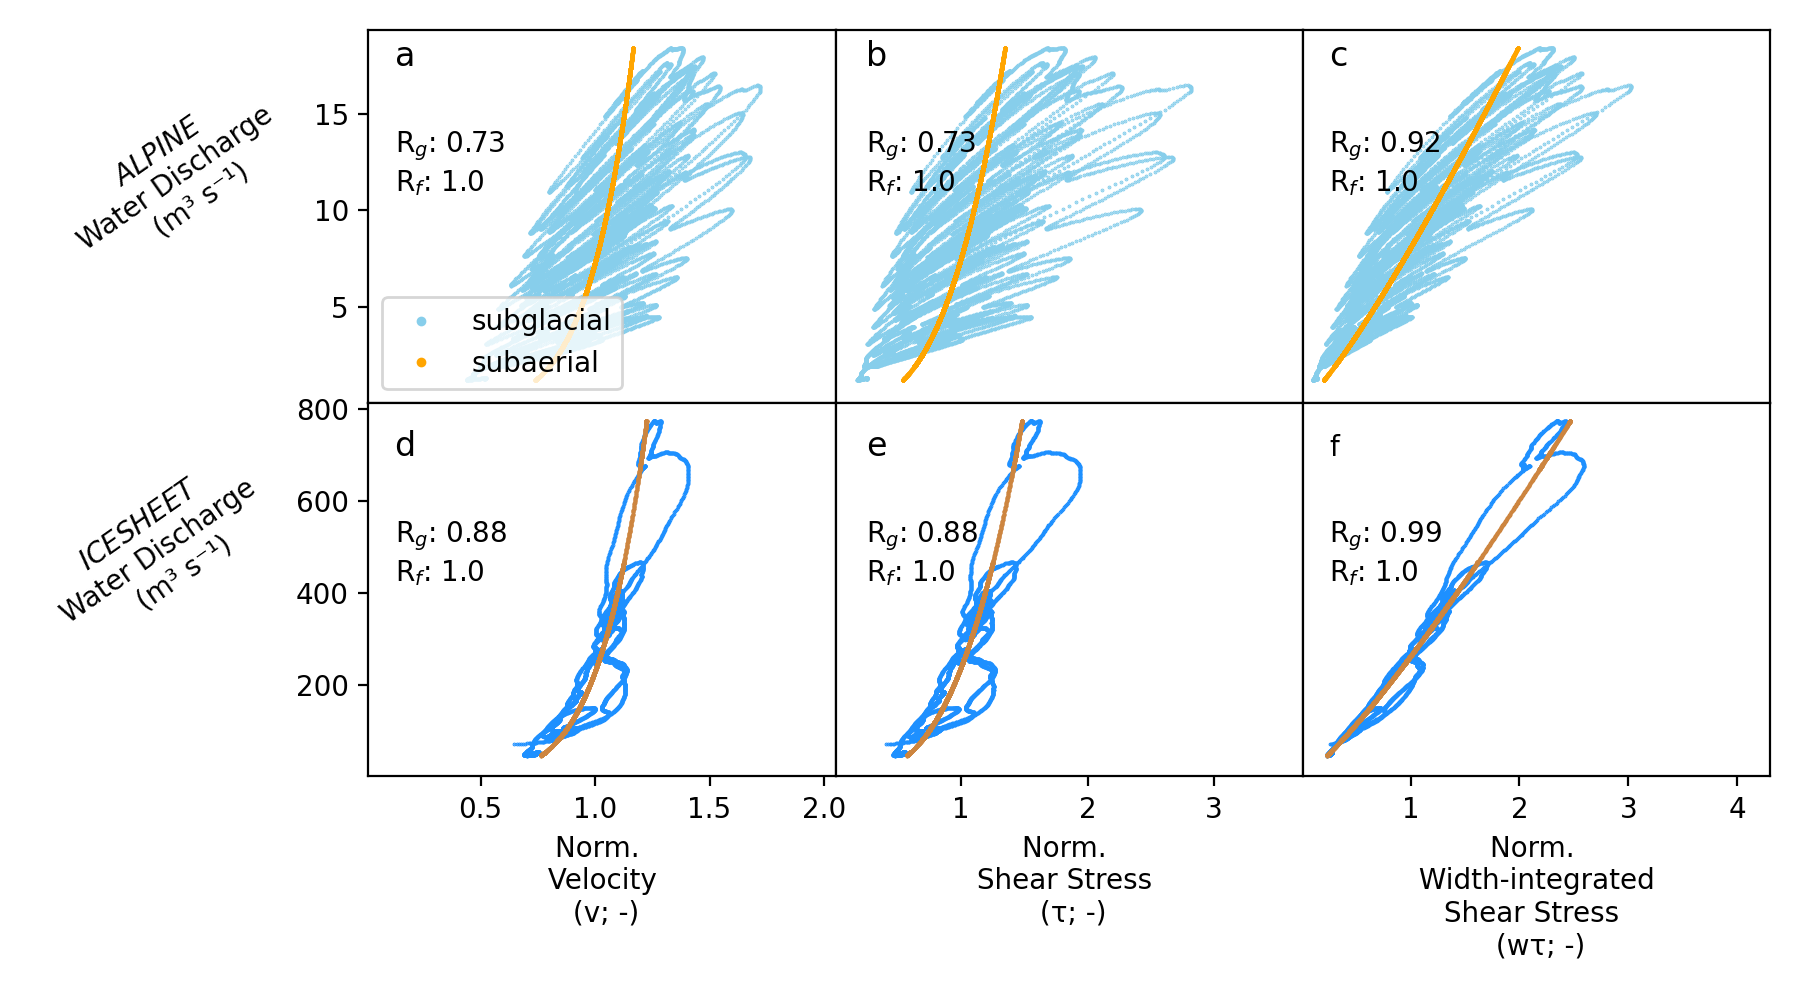
\includegraphics[width=0.7\linewidth]{Fig3_12hr.png}
    \caption{As Figure \ref{fig:model_outs}, with $12$ \,\unit{hr} aggregation.}
    \label{fig:model_outs_12hr}
  \end{figure}
\end{center}


\begin{center}
  \begin{figure}[!h]
    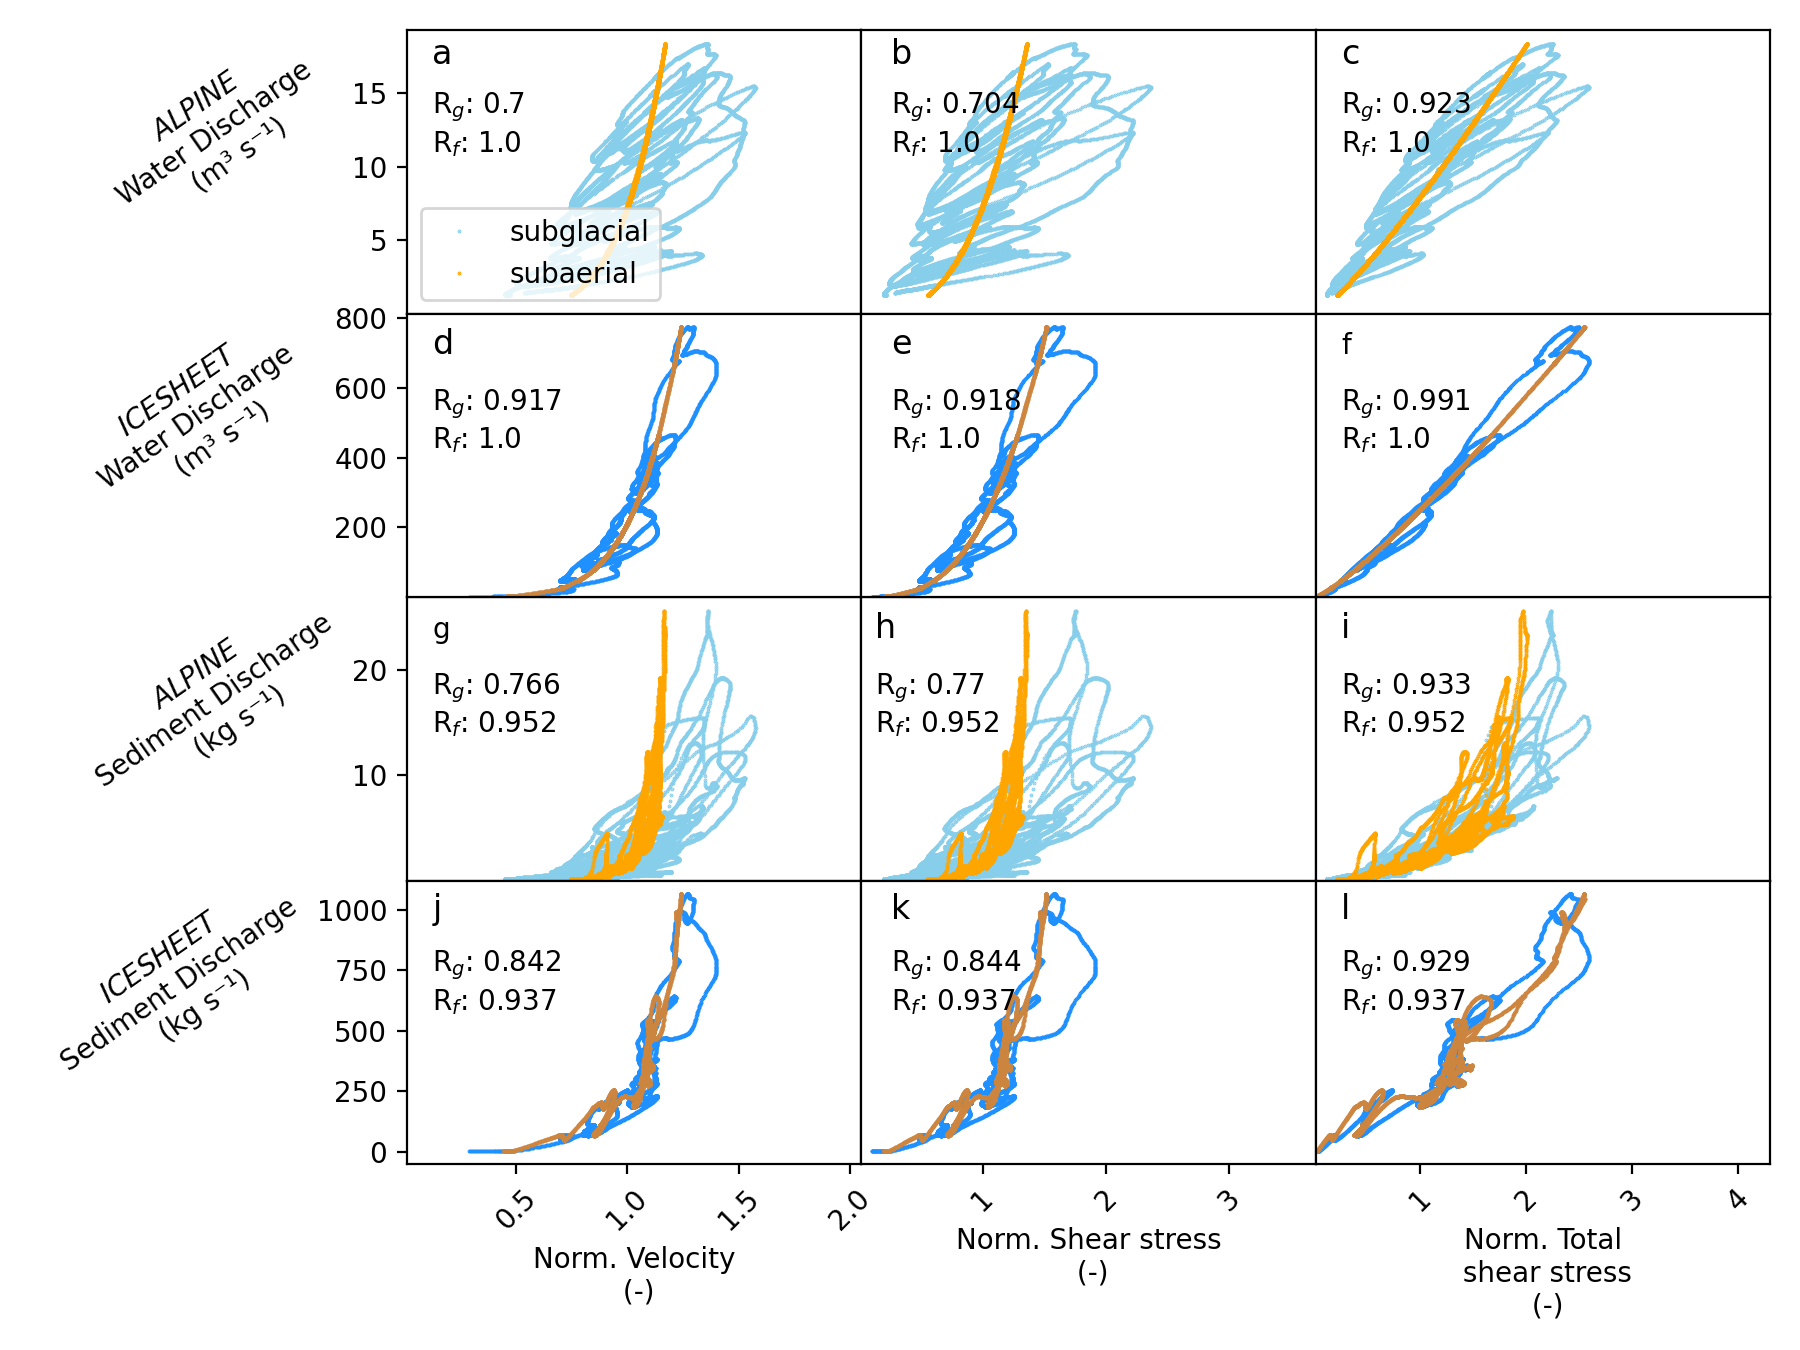
\includegraphics[width=0.7\linewidth]{Fig3_1day.png}
    \caption{As Figure \ref{fig:model_outs}, with $1$ \,\unit{day} aggregation.}
    \label{fig:model_outs_1day}
  \end{figure}
\end{center}


\begin{center}
  \begin{figure}[!h]
    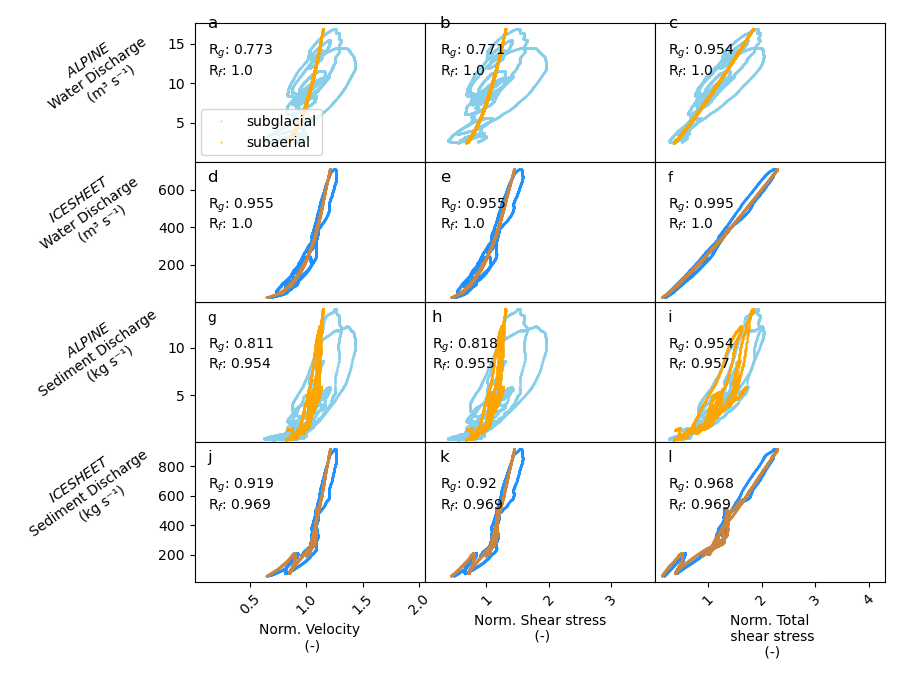
\includegraphics[width=0.7\linewidth]{Fig3_5day.png}
    \caption{As Figure \ref{fig:model_outs}, with $5$ \,\unit{day} aggregation.}
    \label{fig:model_outs_5day}
  \end{figure}
\end{center}

\begin{center}
  \begin{figure}[!h]
    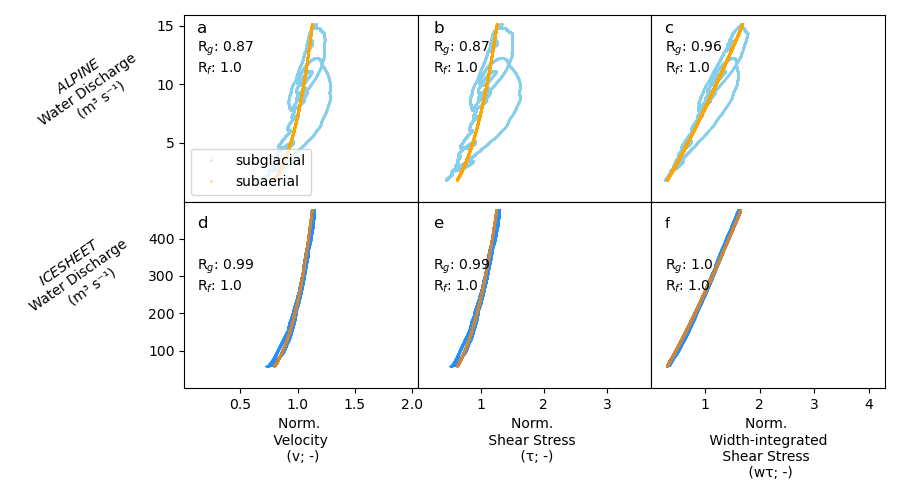
\includegraphics[width=0.7\linewidth]{Fig3_10day.png}
    \caption{As Figure \ref{fig:model_outs}, with $10$ \,\unit{day} aggregation.}
    \label{fig:model_outs_10day}
  \end{figure}
\end{center}

\begin{center}
  \begin{figure}[!h]
    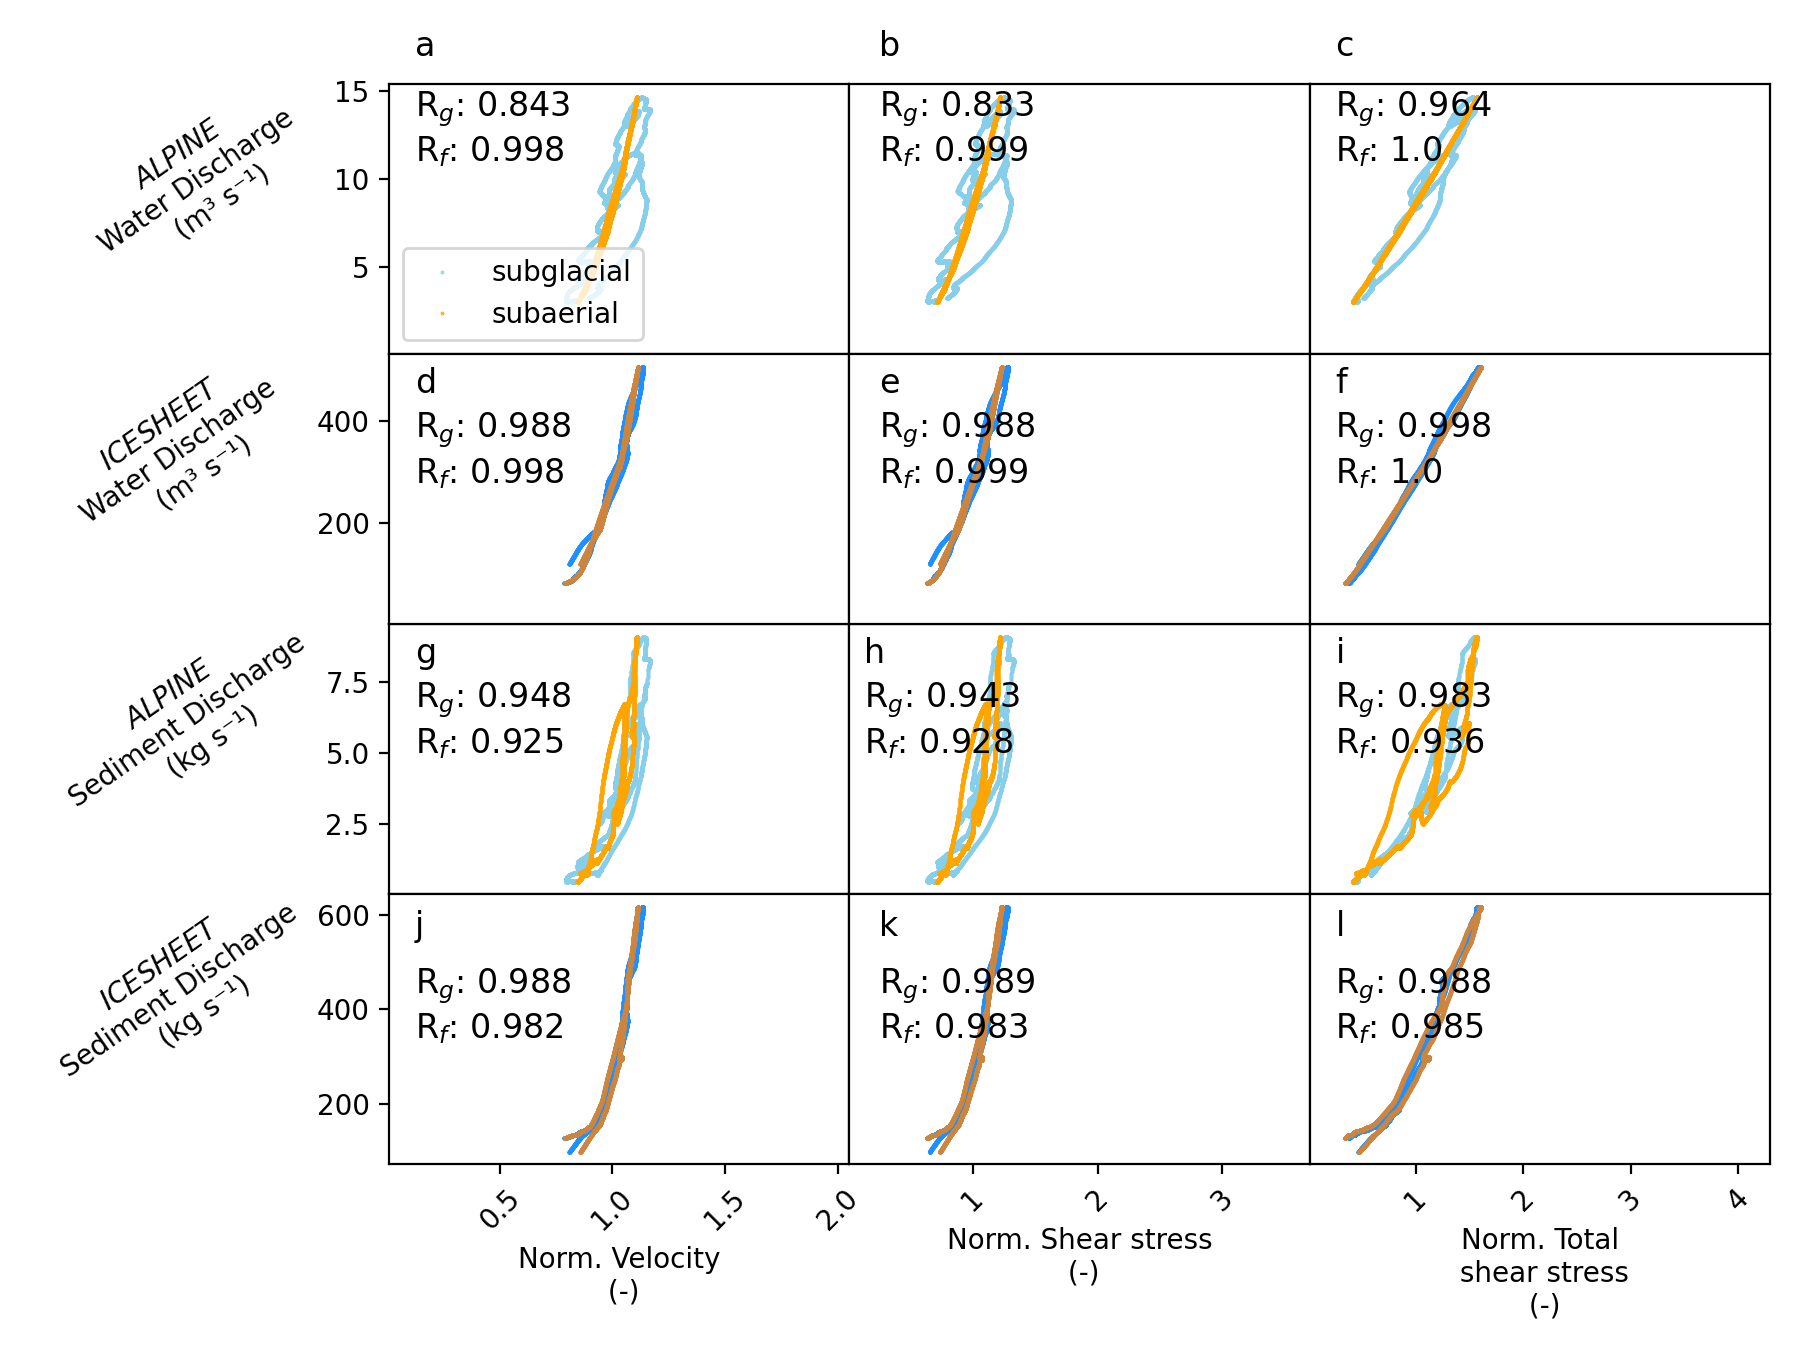
\includegraphics[width=0.7\linewidth]{Fig3_15day.png}
    \caption{As Figure \ref{fig:model_outs}, with $15$ \,\unit{day} aggregation.}
    \label{fig:model_outs_15day}
  \end{figure}
\end{center}
\FloatBarrier



\newpage
\section{Formulas for sediment transport in different drainage regimes}
\label{sect:scaling}

%\mauro{Notation: either use $h$ and $w$ for the river, or otherwise, somehow free $h$. Below I use $H$ and $W$ for now.}

Here three kinds of drainage regimes are examined, namely, subaerial channels, steady-state R-channels \cite{rothlisberger1972}, and pipe-flow (i.e. R-channels which do not have time to adjust their size to discharge conditions).
Here we show how sediment transport capacity scales with respect to a given water discharge and hydraulic gradient for three different transport formulas: Meyer-Peter M\"uller  \cite<MPM;>{meyer1948}, Engelund and Hansen \cite<EH;>{engelund1967}, and Bagnold \cite{bagnold1980}; additionally width-integrated shear stress is assessed, as used as proxy for sediment transport throughout the manuscript.

A few basic hydraulic relations are used in the following.
The Darcy-Weisbach equation can be stated as
\begin{equation}
  \label{eq:DW}
  \Psi \propto f\frac{Q^2}{D_h S^2},
\end{equation}
with $\Psi = \Delta h / l$ the head gradient and friction factor $f$.
The shear stress and stream power are, respectively,
\begin{equation}
    \label{eq:tau-omega}
  \tau \propto f v^2 = f \left(\frac{Q}{S}\right)^2, \quad  \Omega \propto \Psi Q.
\end{equation}
%

Sediment discharge is given by the MPM, EH and Bagnold formulations as
\begin{equation}
  Q_s \propto w\, \tau^{3/2}, \quad Q_s \propto w\, \tau^{5/2}, \quad Q_s \propto w \left(\frac{\Omega}{w}\right)^{3/2} H^{-2/3},
\end{equation}
respectively, for conditions well above the transport onset threshold.

The  subaerial channel is assumed to have a width $w$ much greater than its depth $H$, such that $D_h\approx 4h$, and to have a constant head gradient ($\Psi$) given by the topography.
Further, it is  assumed that its width can be approximated by a relation $w \propto Q^\alpha$ (Equation~\ref{eq:wcf}) with $\alpha\in [0,1]$; typically $\alpha \approx 1/2$ (a so-called regime channel).
End members $\alpha=0$ or $\alpha=1$ correspond a  subaerial channels of constant width (a slot canyon) or depth (no natural equivalent), respectively.
%
For a steady state R-channel, it is assumed that  $\Psi$ is constant (approximated by the gradient of the Shreve \citeyear{shreve1972} potential \footnote{Note that the R-channel model presented above (Eq.~\eqref{eq:dS_dt}--\eqref{eq:dh2wc}), calculates $\Psi$ from the time evolving $S_g$ (Eq.~\eqref{eq:dS_dt}) via the Darcy-Weisbach equation~\eqref{eq:dh} and thus no Shreve approximation is then needed.}) and that $S$ adjusts such that it is in steady state with $\Psi$ and $Q$.
% Conversely, pipe flow has $S$ fixed and $\Psi$ adjusts to satisfy the given $Q$.
%
Pipe flow like conditions occur when a R-channel is subjected to rapid discharge variations such that the channel cannot adjust its size significantly on the time scale of the discharge variations.
In this case, it is assumed that the cross-sectional area $S$ is fixed, and $\Psi$ adjusts to the specified $Q$.
For both R-channel and pipe flow, it is assumed that $D_h \propto S^{1/2}$.

With these assumptions the Darcy-Weisbach equation~\eqref{eq:DW} can be solved for the not-fixed quantity: $H$ for a  subaerial channel, $S$ for a R-channel, and $\Psi$ for pipe-flow.
Then, using equations~\eqref{eq:tau-omega}, the shear stress and stream power can be calculated.
These results are summarised in Table~\ref{tab:eqs1}.
Now width integrated shear stress and sediment transport can be calculated for all regimes and for all transport formulas.  The results of the 12 combinations are presented in Table~\ref{tab:Qs} and also in Table~\ref{tab:Qs2} where the fractions in the exponents are approximately given by decimal numbers for ease of comparison.

Table~\ref{tab:Qs2} shows how the proxy $w\tau$ as well as $Q_s$ of the MPM, EH and Bagnold sediment transport formulas scale with respect to $Q$, $\Psi$ or $S$ for the three different regimes and for different $\alpha$.
Remarkably, the Bagnold formula has a negative exponent for $f$ in all but the pipe-flow regime, which seems rather unexpected.
The total transport formula EH gives a slightly stronger dependence on all variables as should be expected due to the larger exponent on $\tau$ of $\frac{5}{2}$ versus  $\frac{3}{2}$  for the others.
Albeit, the sediment transport response in pipe-flow for the Bagnold case is close to EH.
Conversely, the sediment transport proxies $w_g\,\tau_g$ \& $w_f\,\tau_f$ used within this publication scale only as $Q^2$ for pipe-flow, whereas the transport scales at least with $Q^3$.
The exponent for the width scaling $\alpha$ only impacts relationship between sediment transport and water discharge in the EH relation in any meaningful way.
However, for the value of $\alpha$ around $\frac{1}{2}$ (a value appropriate for most streams), the exponent on $Q$ for EH is only slightly above what the other transport relations give.

The sediment discharge in the steady state R-channel scales very similarly to the  subaerial channel case for all relations and virtually identically for the $\alpha=0.5$ case.  However, note that the head gradients $\Psi$ are likely higher for comparable $Q$ in an ice-sheet marginal or alpine glacier setting than in a  subaerial channel, as is well described in \citeA{alley1997}, and thus transport rates may still be much higher in a steady state R-channel.

Furthermore, R-channels will rarely operate in steady state as variations in discharge, in particular on the diurnal timescale or the timescale of severe rain or melting events, are too fast for such a channel to reach a steady state.
In such cases they operate more like a pipe of fixed cross-section \cite<e.g.>{gimbert2016}.
Table~\ref{tab:Qs2} shows that in such a situation, the sediment transport scales much more severely with discharge, with the exponent on $Q$ being between $3$ and $5$, compared to the other two regimes when that exponent is at most $1.7$ (Table~\ref{tab:Qs2}).
Thus fluctuations of discharge on short timescales (on the order of a day) have the potential to cause conditions with very high sediment transport capacities.


\begin{table}
  \caption{Relations for hydraulic variables for the three drainage regimes:  subaerial channels, R-channel and pipe-flow.  Darcy-Weisbach equation is abbreviated with ``D-W'', and stream power with ``Stream p.''. }
  \small
  \label{tab:eqs1}
\begin{tabular}{llllll}
  Regime & Fixed & Determined via D-W
   & Additional relations & Shear stress & Stream p.\\
& & (Equation~\ref{eq:DW})  &  &  \(\tau \propto\) & \(\Omega \propto\)\\
\hline
  Subaerial & \(\Psi\) & \(H \propto f^{1/3}\, Q^{2/3-2\alpha/3} \, \Psi^{-1/3}\) & \makecell{\(w\,\propto Q^\alpha\) \\ \(S=wH\) \\ \(D_h\propto H\)} & \(f^{1/3} Q^{2/3-2\alpha/3}  \Psi^{2/3}\) & \(Q\, \Psi\)\\
  R-channel & \(\Psi\) & \(S\, \propto f^{2/5}\, Q^{4/5} \, \Psi^{-2/5}\) & \(D_h\propto w \propto H \propto S^{1/2}\) & \(f^{1/5} Q^{2/5} \, \Psi^{4/5}\) & \(Q\, \Psi\)\\
Pipe & \(S\) & \(\Psi \propto f \, Q^2\, S^{-5/2}\) & \(D_h\propto w \propto H \propto S^{1/2}\) & \(f Q^2 S^{-2}\) & \(f\, Q^3 S^{-5/2}\)\\
\end{tabular}
\end{table}

\begin{table}
  \caption{Sediment transport proxy ($w\tau$) and rates for the three considered different transport formulas: MPM \cite{meyer1948}, EH \cite{engelund1967}, and Bagnold \cite{bagnold1980}.
  }
  \small
  \label{tab:Qs}
\begin{tabular}{lllll}
 & Width \(\times \,\, \tau\) & MPM & EH & Bagnold\\
 & \(w\, \tau\) & \(Q_s \propto w\, \tau^{3/2}\) & \(Q_s \propto w\, \tau^{5/2}\) & \(Q_s \propto w^{-1/2}\, \Omega^{3/2} H^{-2/3}\)\\
\hline
Subaerial  & \(f^{1/3}\, Q^{2/3+\alpha/3}\,  \Psi^{2/3}\) & \(f^{1/2}\, Q \, \Psi\) & \(f^{5/6}\, Q^{5/3 - 2\alpha/3} \, \Psi^{5/3}\) & \(f^{-2/9}\, Q^{19/18-\alpha/18} \, \Psi^{31/18}\)\\
R-channel & \(f^{2/5}\, Q^{4/5} \, \Psi^{3/5}\) & \(f^{1/2}\, Q \, \Psi\) & \(f^{7/10}\, Q^{7/5}\, \Psi^{9/5}\) & \(f^{-7/30}\, Q^{31/30}\, \Psi^{26/15}\)\\
Pipe & \(f \, Q^2 \, S^{-1}\) & \(f^{3/2}\, Q^3 \, S^{-5/2}\) & \(f^{5/2}\, Q^5\, S^{-9/2}\) & \(f^{3/2} \, Q^{9/2} \, S^{-14/3}\)\\
\end{tabular}
\end{table}

\begin{table}
  \caption{As Table~\ref{tab:Qs} but with the fractional exponents stated as rounded decimal numbers.  For the subaerial regime the exponents are for displayed for the likely width-exponent $\alpha=1$, as well as its end members 0 (slot canyon) and 1 (only width increases and not depth).
  }
  \small
  \label{tab:Qs2}
\begin{tabular}{lllll}
 & Width \(\times \,\, \tau\) & MPM & EH & Bagnold\\
 & \(w\, \tau\) & \(Q_s \propto w\, \tau^{3/2}\) & \(Q_s \propto w\, \tau^{5/2}\) & \(Q_s \propto w^{-1/2}\, \Omega^{3/2} H^{-2/3}\)\\
\hline
Subaerial (\(\alpha=0\)) & \(f^{0.7}\, Q^{0.7}\,  \Psi^{0.7}\) & \(f^{0.5}\, Q \,\,\,\, \Psi\) & \(f^{0.8}\, Q^{1.7} \, \Psi^{1.7}\) & \(f^{-0.2}\, Q^{1.1} \, \Psi^{1.7}\)\\
Subaerial (\(\alpha=0.5\)) & \(f^{0.7}\, Q^{0.8}\,  \Psi^{0.7}\) & \(f^{0.5}\, Q \,\,\,\, \Psi\) & \(f^{0.8}\, Q^{1.3} \, \Psi^{1.7}\) & \(f^{-0.2}\, Q^{1.0} \, \Psi^{1.7}\)\\
Subaerial (\(\alpha=1\)) & \(f^{0.7}\, Q^{1.0}\,  \Psi^{0.7}\) & \(f^{0.5}\, Q \,\,\,\, \Psi\) & \(f^{0.8}\, Q^{0.7} \, \Psi^{1.7}\) & \(f^{-0.2}\, Q^{1.0} \, \Psi^{1.7}\)\\[3pt]
R-channel & \(f^{0.4}\, Q^{0.8} \, \Psi^{0.6}\) & \(f^{0.5}\, Q \,\,\,\, \Psi\) & \(f^{0.7}\, Q^{1.4}\, \Psi^{1.8}\) & \(f^{-0.2}\, Q^{1.0} \, \Psi^{1.7}\)\\
Pipe & \(f \,\quad Q^{2\phantom{.0}} \, S^{-1}\) & \(f^{1.5}\, Q^3 \, S^{-2.5}\) & \(f^{2.5}\, Q^{5\phantom{.0}}\, S^{-4.5}\) & \(f^{1.5} \,\,\,\,\, Q^{4.5} \, S^{-4.7}\)\\
\end{tabular}
\end{table}

\end{document}


% Graveyard
% Additionally uggest that additional processes and erosional hiatuses may further complicate signals of sediment discharge from glaciers in response to climate \cite{jansson2005,ganti2016}.
% Sediment discharge records have been used to establish the relationship, or lack thereof, between climate forcing and glacial erosion \cite<e.g.>{koppes2009a,ganti2016,willenbring2016,mariotti2021}.
% The variable relationship between water discharge and subglacial sediment transport capacity presented here mostly applies to the daily- to weekly-time scales controlling the size of subglacial channels (Figure~\ref{fig:multi_run}).
% Yet, identifying climatic effects in sediment transport from the transport-limited component of glacier-sedimentary systems may require higher thresholds of water discharge compared to subaerial systems when water discharge varies substantially over short timescales \cite<Figure~\ref{fig:Qw_vari}; >{tofelde2021}. \mauro{I don't understand the last two sentences.}
%Furthermore evaluating the different variability in sediment transport characteristics across timescales can help inform the sediment transport processes omitted from daily or week values of water discharge..